% -- Présentation
% Module : INFO606
% Année  : 2014-2015

% HADJI Monir et MOHIMONT Lucas

\documentclass[handout]{beamer}

% -----
% ----- Preambule
% -----
\usepackage[utf8]{inputenc}
\usepackage[T1]{fontenc}
\usepackage{lmodern}
\usepackage[francais]{babel}

\usetheme{Madrid}
\useoutertheme{infolines}
%\useoutertheme{split}

\setbeamertemplate{headline}
{
  \leavevmode
  \hbox
      {%  Partie gauche : titre de la section
        \begin{beamercolorbox}[wd=.5\paperwidth,ht=2.25ex,dp=1ex,right,rightskip=1em]{section in head/foot}%
          \usebeamerfont{subsection in head/foot}\insertsectionhead
        \end{beamercolorbox}%
        % Partie droite : titre de la sous-section
        \begin{beamercolorbox}[wd=.5\paperwidth,ht=2.25ex,dp=1ex,left,leftskip=1em]{subsection in head/foot}%
          \usebeamerfont{section in head/foot}\insertsubsectionhead
        \end{beamercolorbox}%
      }
      \vskip0pt
}

\setbeamertemplate{blocks}[rounded][shadow=false]

% Pour chaque début de section
\AtBeginSection
{
%  \begin{frame}
  %    \frametitle{Table des matières}
   %   \tableofcontents[currentsection, hideothersubsections]
  %  \end{frame}
}

% Page de garde
\title[Visualisation d'algorithmes intéractifs]{Framework pour la visualisation d'algorithmes intéractifs}
\author[L. Mohimont / M. Hadji]{Lucas Mohimont \& Monir Hadji}
\institute[INFO606]{Licence 3 Info - INFO606 - Projet de programmation\\Resp. Projet : Jean-Charles Boisson\\Resp. Module : Christophe Jaillet}
\date{2014-2015}

% -----
% ----- Debut document
% -----
\begin{document}

% Frame de presentation
\begin{frame}
  \titlepage
  \begin{center}
    \includegraphics[width=3cm]{contents/urca.jpg}
  \end{center}
\end{frame}

% Frame de table des matières

\begin{frame}
  \frametitle{Framework pour la visualisation d'algorithmes intéractifs}

  \begin{block}{Cela doit permettre de}
    \begin{itemize}
    \item Pouvoir visualiser des structures de données
    \item Pouvoir visualiser des algorithmes sur ces structures
    \item Pouvoir intéragir avec le framework
    \end{itemize}
  \end{block}
\end{frame}

\begin{frame}
  \frametitle{Table des matières}
  \tableofcontents[hideallsubsections]
\end{frame}

\section{Choix des technologies}
\begin{frame}
  \frametitle{Visualisation}

  \begin{block}{Possibilités en environnement graphique}
    \begin{itemize}
    \item SDL2
    \item SFML
    \item Qt
    \item GTKmm
    \end{itemize}
  \end{block}

  \begin{block}{Possibilités en environnement graphique}
    \begin{itemize}
    \item SDL2 et SFML pas très approprié pour de l'interface graphique
      \begin{itemize}
      \item Davantage utilisé pour faire du jeu vidéo 2D
      \end{itemize}
    \item GTKmm pas portable, la dernière version pas présente sur Windows
      \begin{itemize}
      \item Difficilement portable
      \end{itemize}
    \item Qt semble un bon compromis
    \end{itemize}
  \end{block}
\end{frame}

\begin{frame}
  \frametitle{Visualisation}
    
  \begin{block}{Contenu 3D}
    \begin{itemize}
    \item Direct3D
      \begin{itemize}
      \item Exclusif à Windows
      \end{itemize}          
    \item OpenGL est multiplateforme
    \end{itemize}
  \end{block}
  
  \begin{exampleblock}{Choix finaux}
    \begin{itemize}
    \item OpenGL pour l'API de rendu
    \item Qt pour l'environnement graphique
    \end{itemize}
  \end{exampleblock}
\end{frame}

\section{Cas de la structure graphe}
\subsection{Problème de placements}
\begin{frame}
  \frametitle{Comment placer les noeuds du graphe ?}

  \begin{block}{Le graphe doit être placé harmonieusement}
    \begin{itemize}
    \item Lisible
    \item Pas de noeuds trop proche (pas de chevauchement)
    \item Pas de noeuds trop éloignés
    \end{itemize}
  \end{block}

  \begin{block}{Plusieurs approches existantes}
    \begin{itemize}
    \item Force directed graph drawing
    \item Spectral graph drawing
    \end{itemize}
  \end{block}
\end{frame}

\begin{frame}
  \frametitle{Force directed graph drawing}

  \begin{block}{Caractéristiques}
    \begin{itemize}
    \item Analogie à un système physique
    \item Résultat trop aléatoire
    \item Placement différent d'une exécution à l'autre
    \end{itemize}
  \end{block}
\end{frame}

\begin{frame}
  \frametitle{Spectral graph drawing}

  \begin{block}{Caractéristiques}
    \begin{itemize}
    \item Calculs de valeurs et vecteurs propres
    \item Placement toujours identique d'une exécution à l'autre
    \end{itemize}
  \end{block}
\end{frame}

\begin{frame}
  \frametitle{Spectral graph drawing}

  \begin{block}{Exemple}
    Résultat obtenu
  \end{block}

  \begin{figure}[ht]
    \begin{center}
      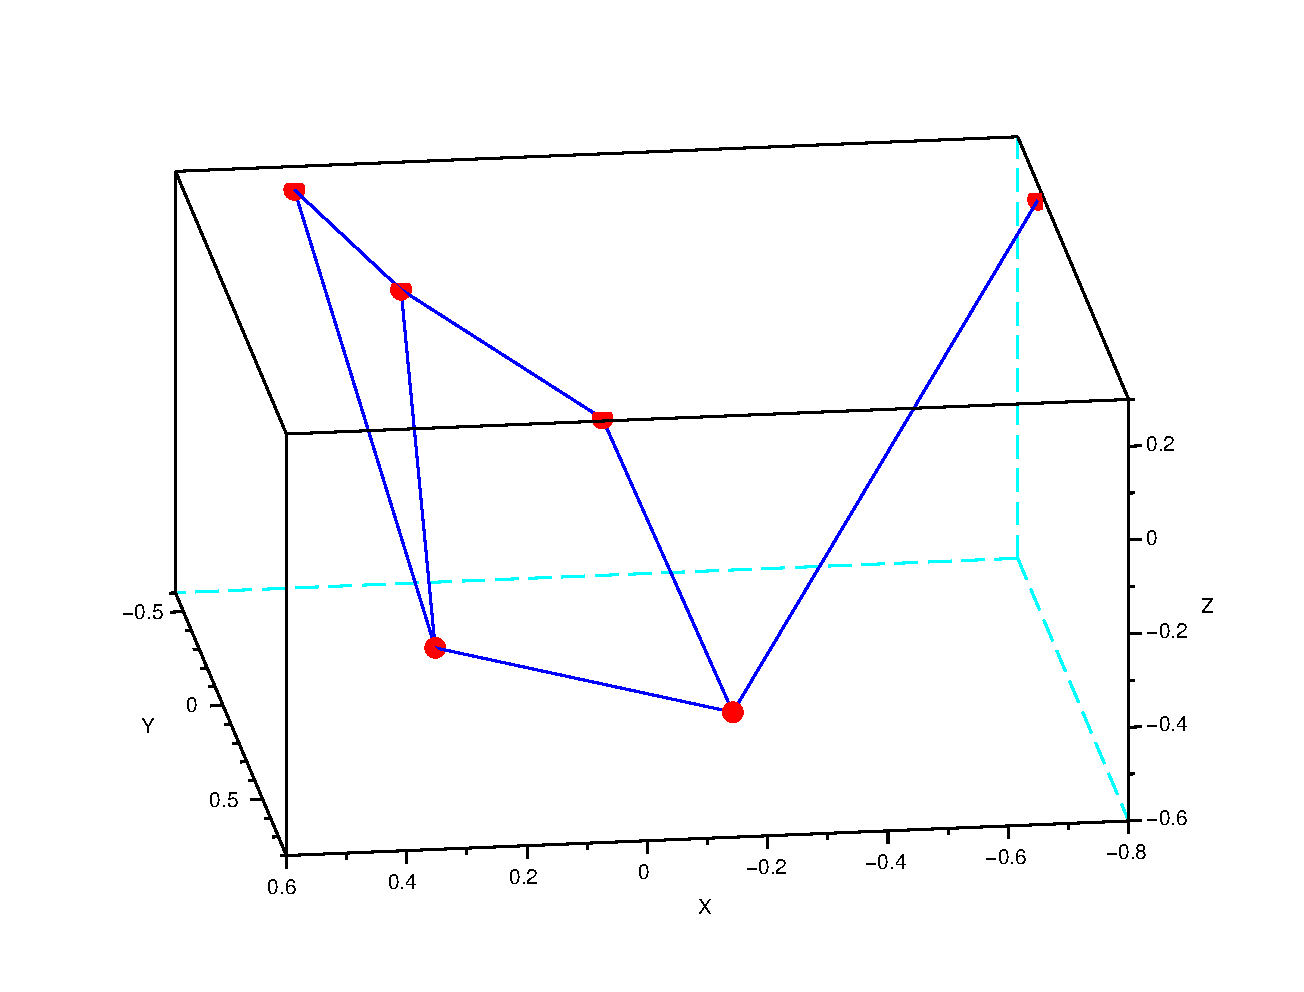
\includegraphics[scale=0.3]{contents/grefsci}
    \end{center}
    \caption{Représentation 3D du graphe de référence sur Scilab}
    \label{fig:G3D}
  \end{figure}
\end{frame}

\begin{frame}
  \frametitle{Comment représenter les noeuds ?}

  \begin{block}{Comment représenter les noeuds ?}
      \begin{itemize}
      \item Impossibilité de visualiser de simple algorithme
      \item Impossibilité de visualiser le noeud courant
      \item Obligation d'ajouter une visualisation des noeuds
      \end{itemize}
  \end{block}
\end{frame}

\begin{frame}
  \frametitle{Comment visualiser un algorithme sans noeuds ?}

  \begin{block}{Ajout de données 3D représentant les noeuds}
    \begin{itemize}
    \item Couleur
    \item 3D (au format Collada .dae)
    \end{itemize}
  \end{block}

  \begin{figure}[h]
    \begin{center}
      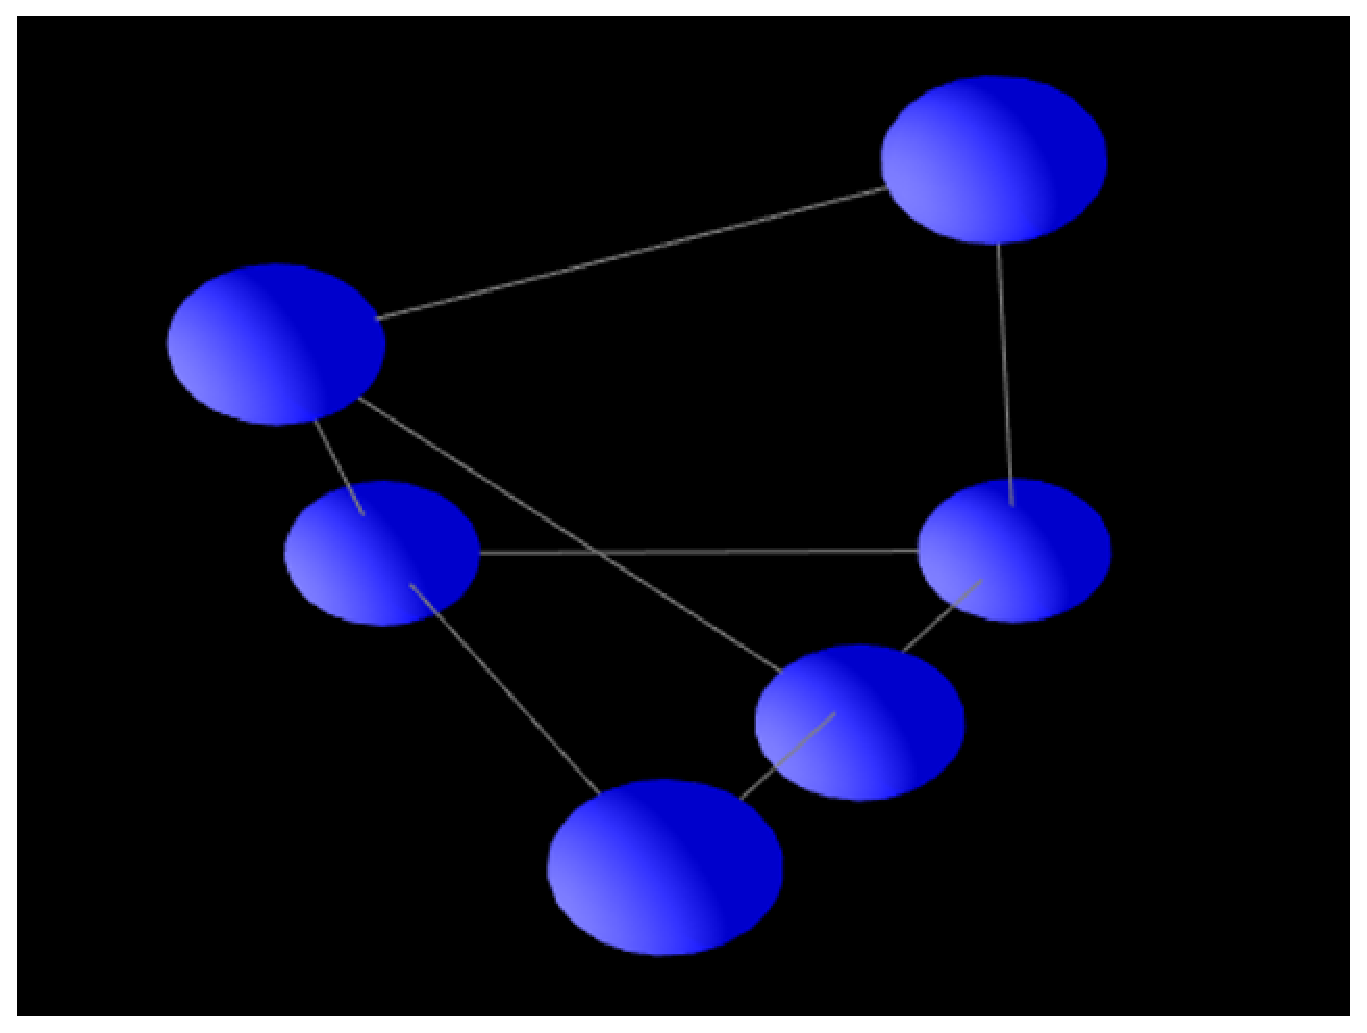
\includegraphics[scale=0.3]{contents/gnode}
    \end{center}
    \label{fig:gnode}
  \end{figure}
\end{frame}

\begin{frame}
  \frametitle{Problème pouvant survenir}

  \begin{block}{Problème de dimension}
    \begin{itemize}
    \item Problème: Si le modèle 3D a une taille trop grande par rapport aux tailles des arêtes
    \item Solution: Calcul de la plus petite norme
    \end{itemize}
  \end{block}

  \begin{figure}[h]
    \begin{center}
      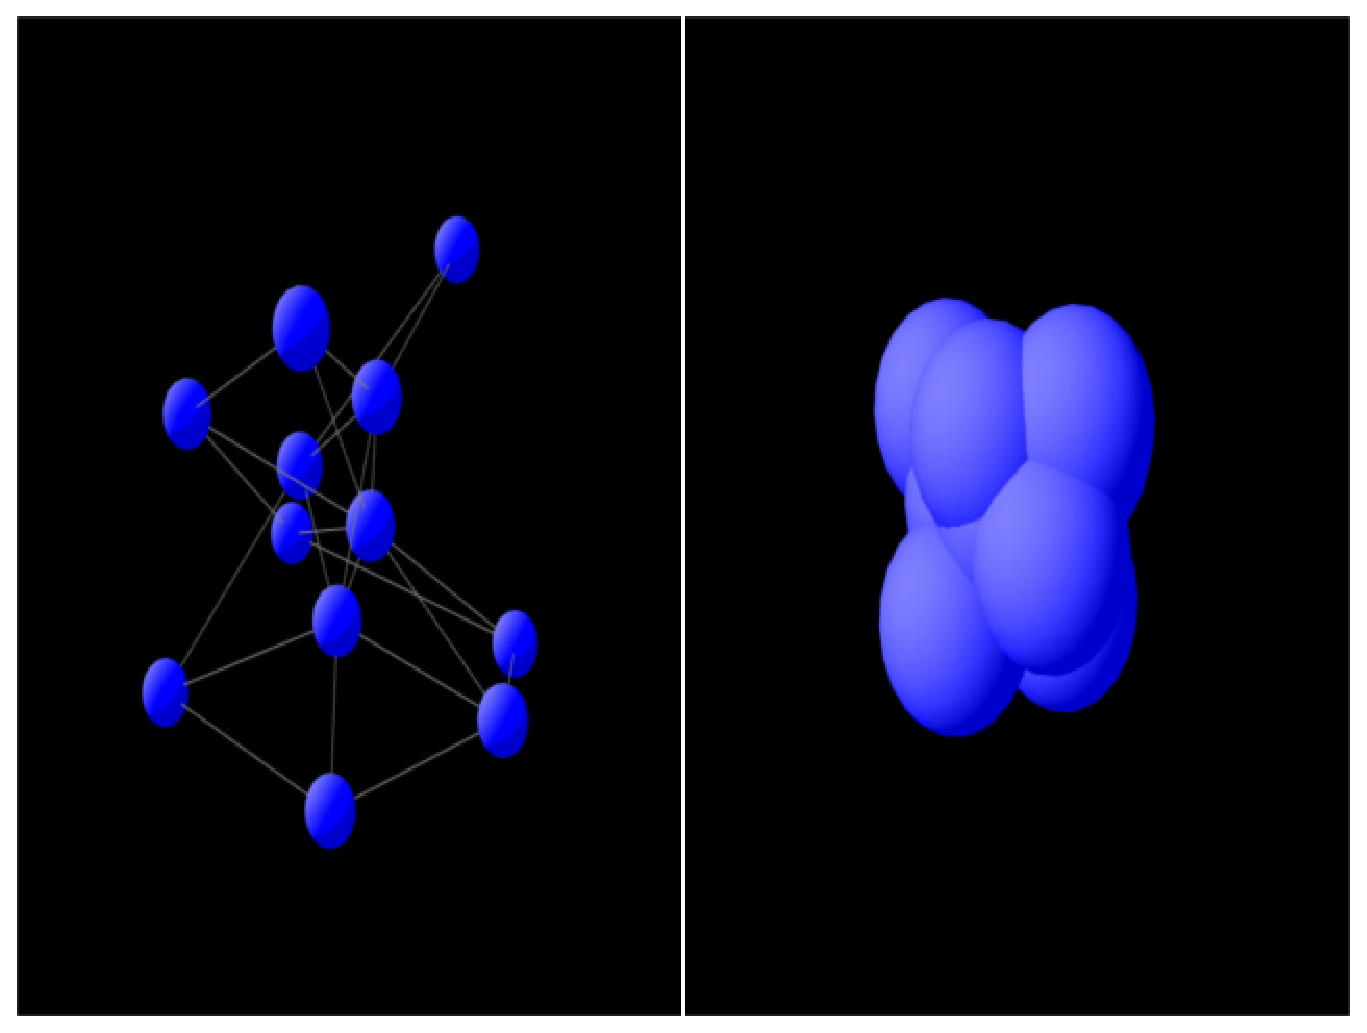
\includegraphics[scale=0.3]{contents/pb2node}
    \end{center}
    \caption{Problème de rendu : dimensions trop grande}
    \label{fig:pb2node}
  \end{figure}
\end{frame}

\begin{frame}
  \frametitle{Intéraction utilisateur}

  \begin{block}{Ajout d'une gestion de la caméra géré à la souris}
    \begin{itemize}
    \item Caméra trackball
    \item Utilisé dans Google Earth
    \item Caméra fixe, rotation de la scène
    \end{itemize}
  \end{block}
\end{frame}

\begin{frame}
  \frametitle{Comment identifier les noeuds ?}

  \begin{block}{Ajout d'identifiant de noeuds}
    \begin{itemize}
    \item Obligation d'ajout de label pour identifier les noeuds
    \item Rectangle avec texture dynamique
    \item Translation du repère vers les coordonnées du noeuds
    \item Dessin du rectangle texturé
    \end{itemize}
  \end{block}
\end{frame}

\begin{frame}
  \frametitle{Comment identifier les noeuds ?}
  \begin{block}{Exemple}
    Résultat obtenu
  \end{block}

  \begin{figure}[h]
    \begin{center}
      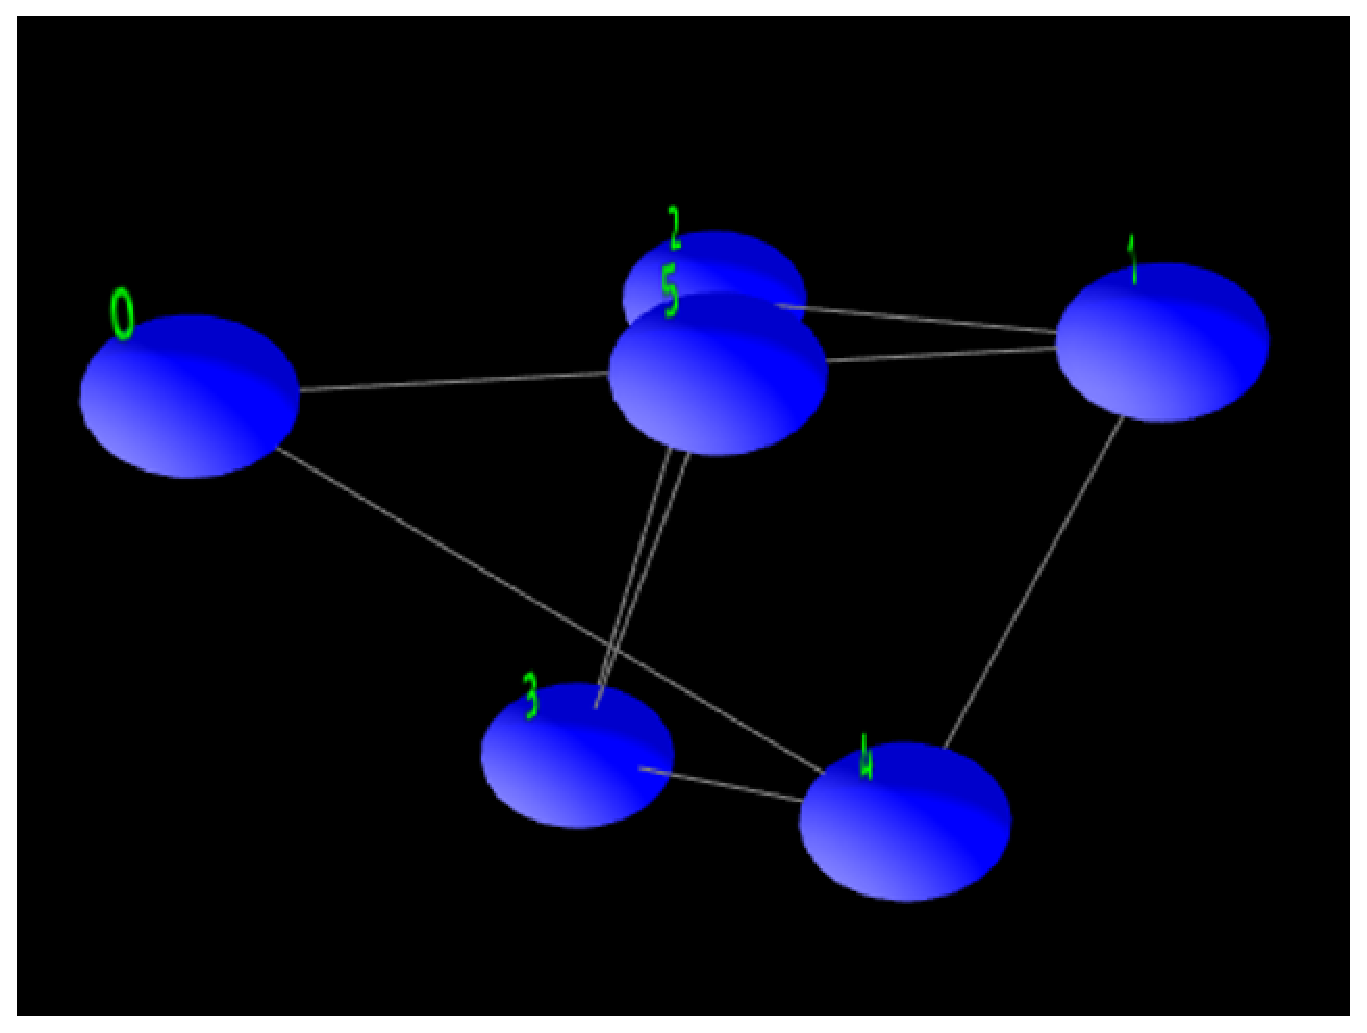
\includegraphics[scale=0.3]{contents/tnode}
    \end{center}
    \caption{Problème de rendu: texte pas toujours face à la caméra si rotation de la scène}
    \label{fig:tnode}
  \end{figure}
\end{frame}

\begin{frame}
  \frametitle{Comment faire en sorte que le texte soit toujours face à la caméra ?}
  \begin{block}{Texte toujours face à la caméra}
    Utilisation du billboarding
  \end{block}

  \begin{block}{Billboarding}
    \begin{itemize}
    \item Rotation du repère
    \item Translation du repère
    \item On supprime la rotation du repère
    \item On dessine le modèle
    \end{itemize}
  \end{block}
\end{frame}

\begin{frame}
  \frametitle{Billboarding}
  \begin{block}{Exemple d'application}
    Très utilisé dans le jeu vidéo
  \end{block}

  \begin{figure}[ht]
    \begin{center}
      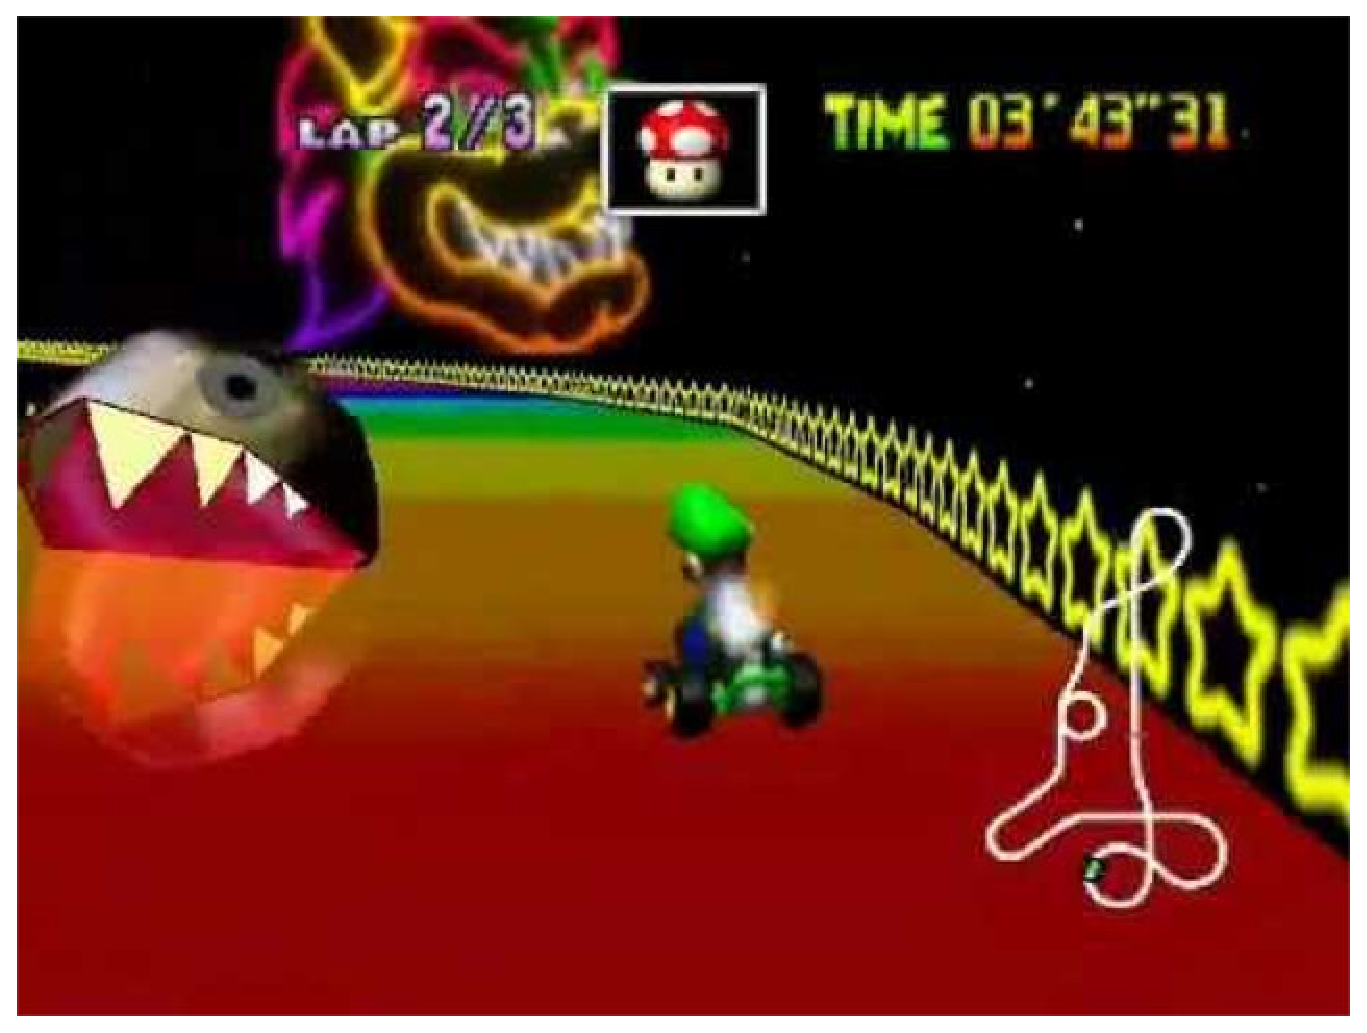
\includegraphics[scale=0.3]{contents/mk64}
    \end{center}
    \caption{Utilisation du billboarding dans \bsc{Mario Kart 64}}
    \label{fig:mk64}
  \end{figure}
\end{frame}

\begin{frame}
  \frametitle{Comment faire en sorte que le texte soit toujours face à la caméra ?}
  \begin{block}{Texte toujours face à la caméra}
    Rendu obtenu
  \end{block}

  \begin{figure}[ht]
    \begin{center}
      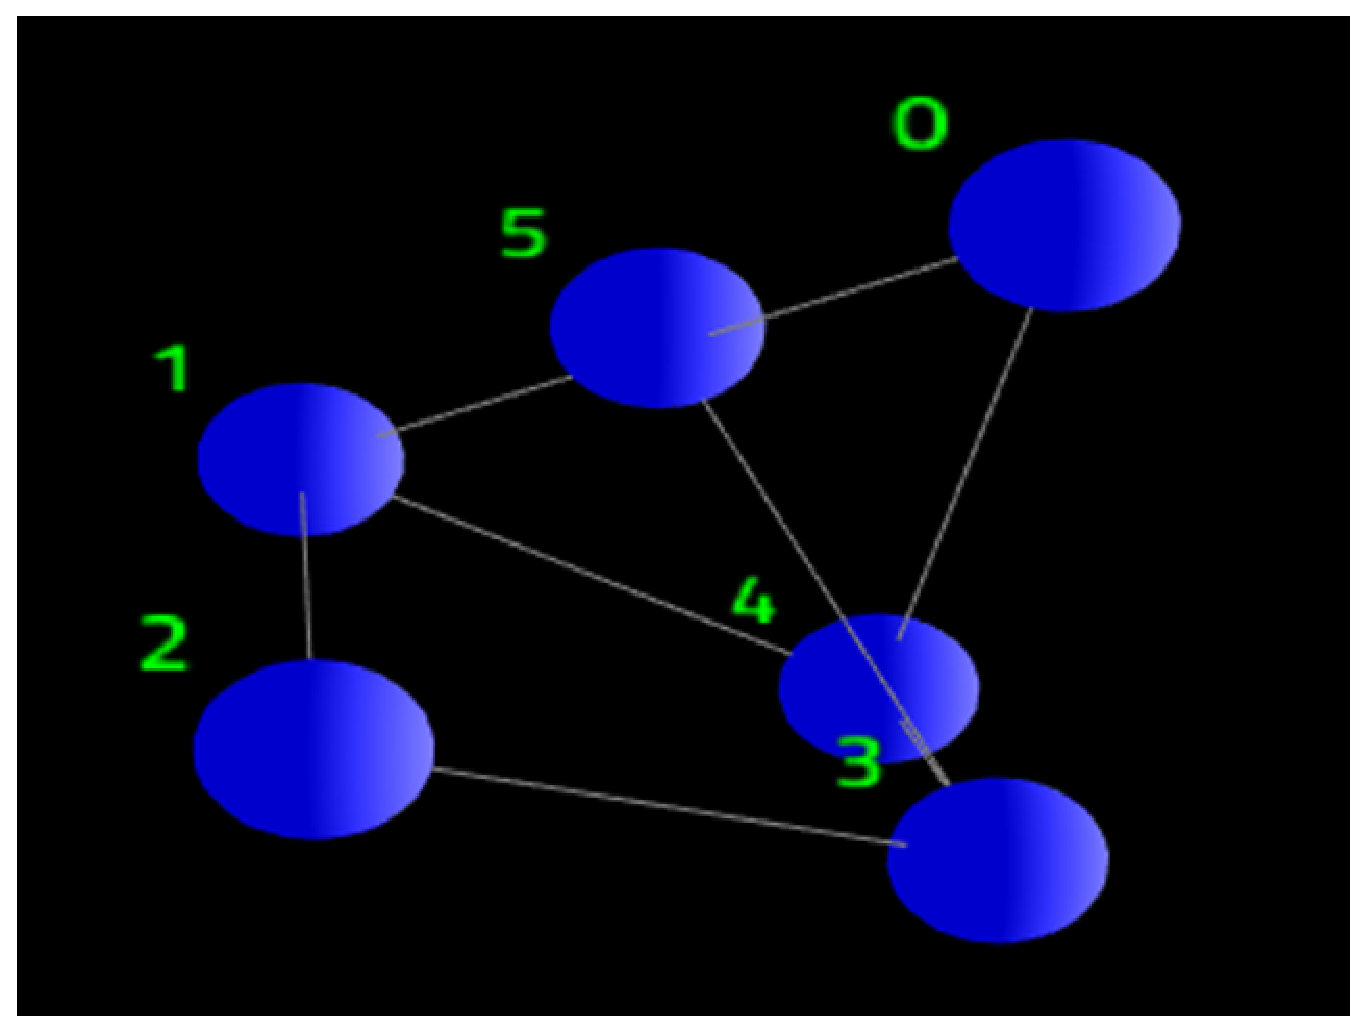
\includegraphics[scale=0.2]{contents/tnode_bb}
    \end{center}
    \caption{Texte avec billboarding}
    \label{fig:tnode_bb}
  \end{figure}
\end{frame}

\begin{frame}
  \frametitle{Comment visualiser l'exécution d'un algorithme}
  \begin{block}{Typage de noeuds}
    \begin{itemize}
    \item On associe un type enum à chaque noeuds
    \item Chaque type enum est associé à un ensemble de donnée de rendu
    \item Modification du type enum des noeuds durant l'exécution de l'algorithme
    \end{itemize}
  \end{block}
\end{frame}

\begin{frame}
  \frametitle{Conclusion et perspectives}
  \begin{block}{Prototype de framework}
    \begin{itemize}
    \item Permet l'ajout de structure de donnée
    \item Permet l'ajout de structure 3D
    \item Permet une visualisation élementaire de l'exécution d'un de ses algorithmes
    \end{itemize}
  \end{block}

  \begin{block}{Perspectives}
    \begin{itemize}
    \item Porter le projet sur OpenGL ES et/ou WebGL
    \item Adaptation du projet en programme éducatif
    \end{itemize}
  \end{block}

\end{frame}

\begin{frame}
  \frametitle{}

  \begin{block}{}
    \begin{center}
      Merci pour votre attention\\
      Des questions ?
    \end{center}
  \end{block}
\end{frame}

\subsection{Problème d'intéraction}

\end{document}
